%&tex

\chapter{Experiments and benchmarks}\label{chp:benchmarks}

In this chapter we apply our model on an artificial self-driving dataset, running several
experiments and measuring how good our models perform with each setup. We first describe the
different configurations we use for training and testing. We then show results on accuracy for each
of the models and pre-processing transformations. Finally we show how fast each model is.

\section{Pre-processing}

Before training and inference, we apply different image transformations to the dataset. As
mentioned in~\autoref{chp:modelling}, we use three main transformations: binarization, quantization
and equalization.

\subsection{Binarization}


\subsection{Quantization}

The Gens-Domingos algorithm, as mentioned in~\autoref{chp:structure}, has two main steps: a
clustering phase and an independency test part. Our independency test implementation in specific
uses the standard G-test statistical independence test based on contingency tables, where each
frequency of the categories of each two variables are laid out on a matrix and their likelihood
ratio are computed. This test takes time $\bigo(n m)$, where $n$ and $m$ are the number of
categories of each variable, and grows fast with $n$ and $m$. We empirically found that when
$\max\{n,m\}$ is relatively big (in our experiments 16 was considered as such) both accuracy and
speed were negatively affected.

A possible explanation for this is the low number of pixel intensity values for too extreme values.
For instance, there are fewer samples where pixels are either too bright or too dark,
as~\autoref{fig:hist-orig} shows.

\begin{figure}[h]
  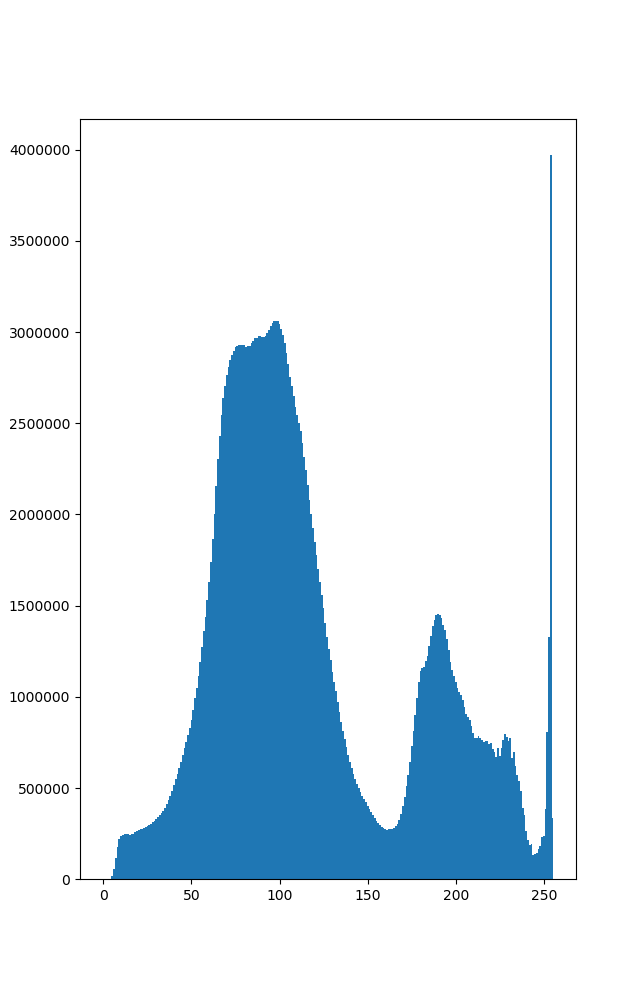
\includegraphics[scale=0.3]{imgs/hist_8.png}
  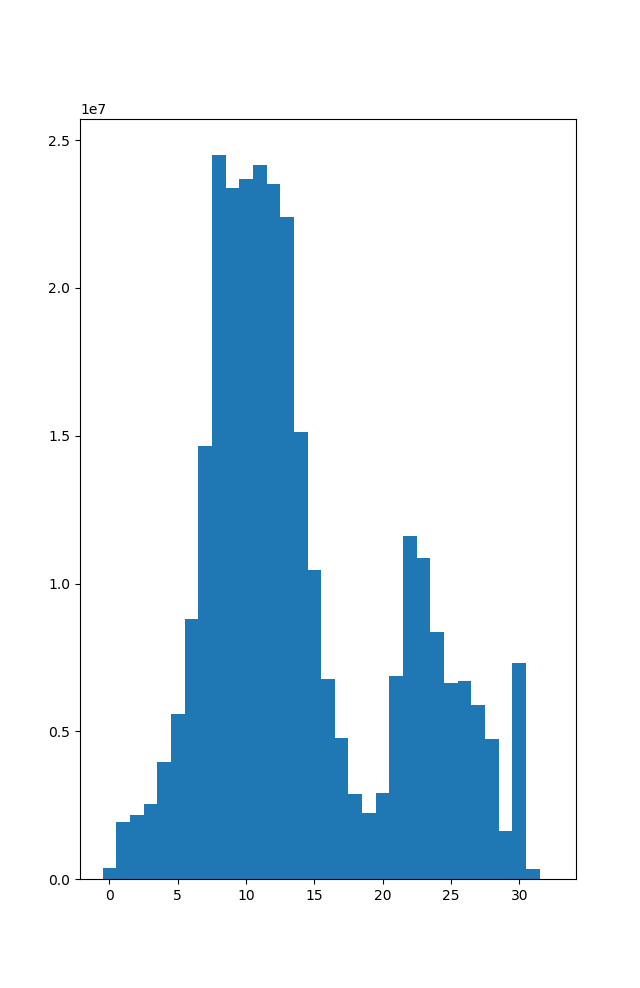
\includegraphics[scale=0.3]{imgs/hist_5.png}
  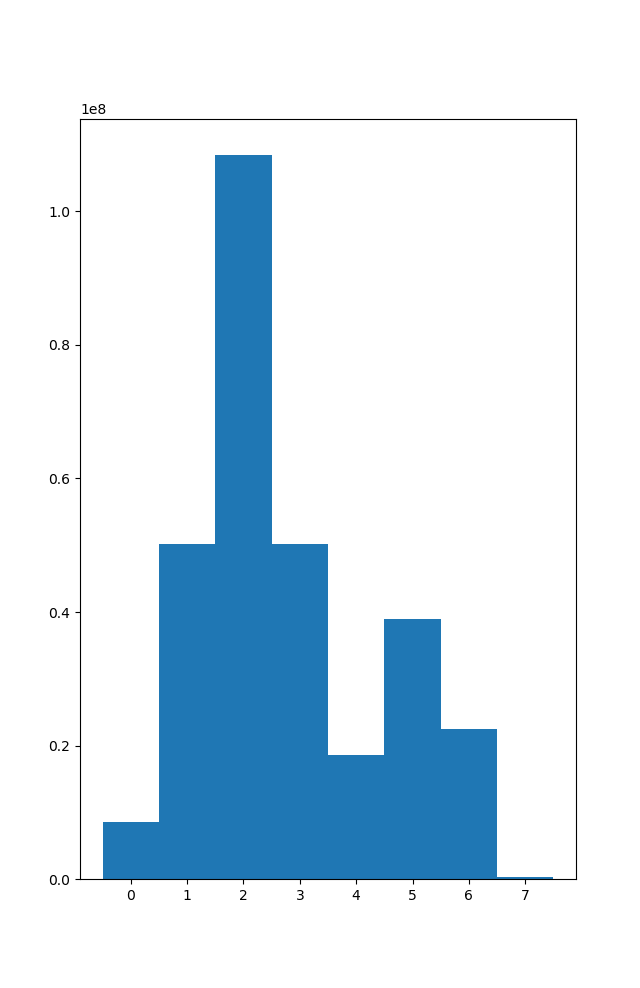
\includegraphics[scale=0.3]{imgs/hist_3.png}
  \caption{Histogram for dataset pixel values on 8-bit, 5-bit and 3-bit image
    resolutions.\label{fig:hist-orig}}
\end{figure}

Although quantizing the dataset proved to be a significant improvement in accuracy to the model
(from $\approx$35\% to 75\%), the issue of fewer, near zero, samples for particular values still
haunted our Gens-Domingos implementation.

We faced two possible solutions to this problem. Either implement an exact independence test, such
as the Fisher exact test (\cite{fisher-exact}), or perform equalization on the dataset. The former
was unfortunately not an option, as we found that there were no libraries in Go or C that provided
a general case implementation of the Fisher exact test, and implementing our own within our time
constraints was out of question. We chose the latter, applying histogram equalization on the entire
dataset.

\subsection{Equalization}

Equalization was done using OpenCV. We attempted two methods of histogram equalization: traditional
equalization through brightness and contrast normalization, and Contrast Limited Adaptive Histogram
Equalization (CLAHE). We found that the CLAHE method resulted in images that were very similar to
the output of the traditional method. Since these transformations are also expected to be applied
on-the-fly during inference, we chose the standard equalization for its speed.
\autoref{fig:hist-eq} shows how the dataset pixel histogram looks like after equalization.

\begin{figure}[h]
  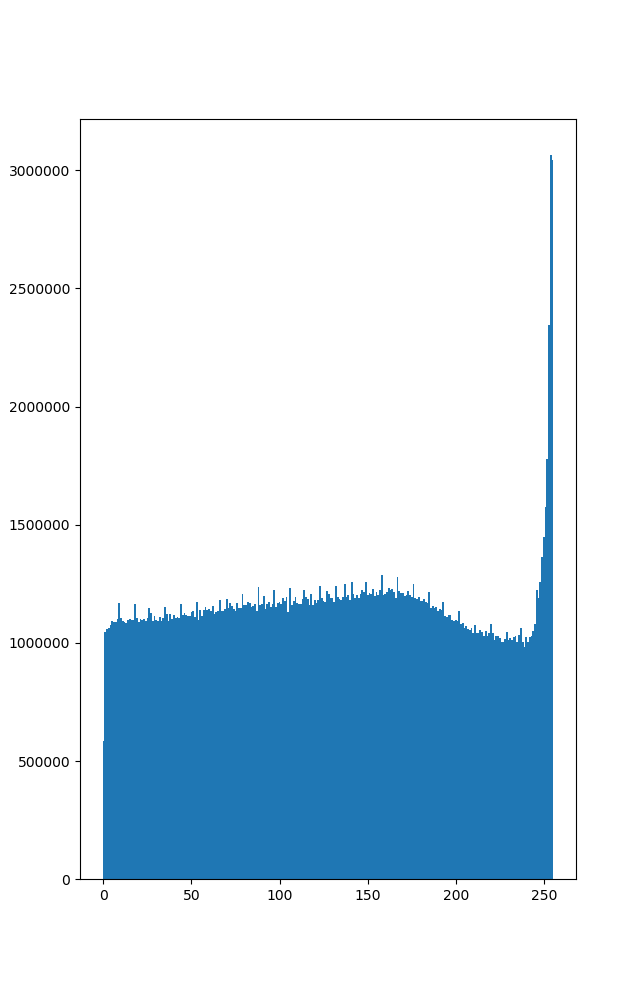
\includegraphics[scale=0.3]{imgs/hist_8_eq.png}
  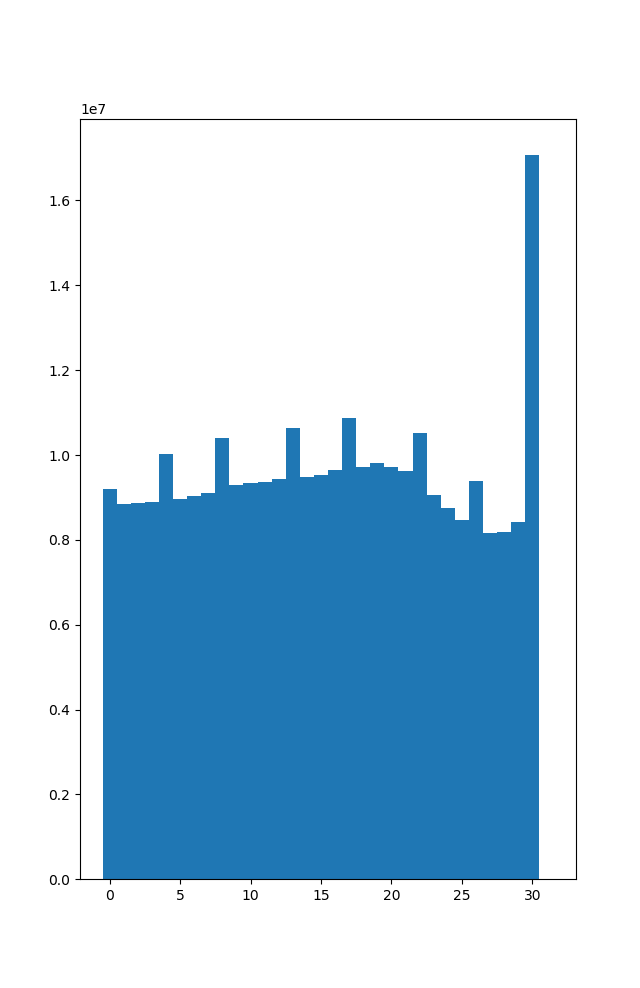
\includegraphics[scale=0.3]{imgs/hist_5_eq.png}
  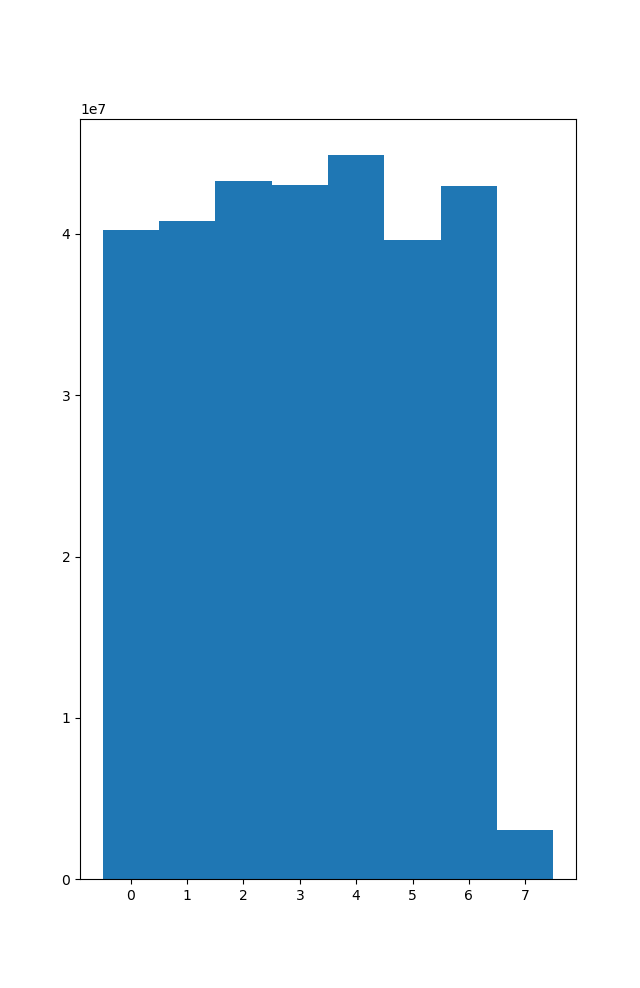
\includegraphics[scale=0.3]{imgs/hist_3_eq.png}
  \caption{Histogram for equalized dataset with 8-bit, 5-bit and 3-bit image
  resolutions.\label{fig:hist-eq}}
\end{figure}

When coupling quantization and equalization, we were able to achieve $\approx$78\% accuracy.
Interestingly, these transformation proved to be harmful for the Dennis-Ventura architecture. In
fact, the structure yielded better results with higher resolutions compared to lower. Equalization
also had little to no effect on this architecture, increasing accuracy in 1\% or 2\%. We attribute
this phenomenom to the classification architecture we discussed in~\autoref{chp:structure}. Since
each sub-SPN is essentially modelling each class as a separate, independent image model to the
other classes, the more details in the image, the easier the model can distinguish from other label
images. Furthermore, since the Dennis-Ventura algorithm does not need to run an independence test,
it does not suffer from its drawbacks.

\section{Setups}

\section{Accuracy}

\section{Speed}
